\section{Przeprowadzone eksperymenty} \label{results}
Niniejszy rozdział opisuje przeprowadzone eksperymenty w~ramach których autor starał się ocenić jak~bardzo sprawdzane metody są w~stanie pomóc w~uzyskaniu wyższej skuteczności w~przypadku uczenia maszynowego. 

\subsection{Sztuczne powiększanie zbioru danych}
\subsubsection{Opis problemu}
Eksperyment sztucznego powiększania danych został przeprowadzony w~oparciu o~konkurs ,,Dogs vs. Cats'' opublikowany w~serwisie Kaggle.\footnote{\label{myfootnote1}\url{https://www.kaggle.com/c/dogs-vs-cats}} Zadaniem uczestników było stworzenie systemu, który~jest w~stanie rozwiązać problem rozpoznawania psów i~kotów na~obrazie. Udostępniona została baza danych 25000 sklasyfikowanych obrazów o~różnych rozmiarach. Mały wycinek udostępnionych danych został przedstawiony na~rysunku \ref{catsdogs}. W~celu ewaluacji stworzonego modelu udostępniony był zbiór 12500 niesklasyfikowanych obrazów. Najlepsze rezultaty uczestnicy otrzymywali przy użyciu głębokich sieci neuronowych i~także ta metoda została wykorzystana w~tej pracy. Zwycięzca pierwszej edycji konkursu uzyskal skuteczność 98,9\%\footnote{\label{myfootnote2}\url{https://plus.google.com/+PierreSermanet/posts/GxZHEH9ynoj}} korzystając właśnie z~głębokich sieci neuronowych. Autor najlepszego rozwiązania, oprócz posłużenia się całym zbiorem opublikowany przez~serwis Kaggle, dodatkowo wykorzystał inny zbiór danych~-~ILSVRC12\footnote{\url{http://www.image-net.org/challenges/LSVRC/2012/results.html}} - w~celu wstępnego uczenia sieci, co daje dobrą podstawę do~treningu modelu dla docelowego zadania. W~przeprowadzonych obliczeniach, dotyczących niniejszej pracy, nie został jednak wykorzystany cały zbiór ze~względu na~bardzo długi czas wykonania programu. Celem tego eksperymentu było zbadanie poprawy klasyfikacji przy użyciu sztucznego powielania danych. Uczenie sieci przeprowadzone zostało przy użyciu 8000 obrazów, a~z kolei 1000 obrazów przeznaczone zostało do~testowania, co w~żadnym wypadku nie stanowi przeszkody w~osiągnięciu założonego celu tego eksperymentu. Pojedyncze uczenie, wraz~z ewaluacją, trwało około 17 godzin. Każdy obraz podawany do~sieci był 4 razy, co dawało 32000 iteracji przy pojedynczym uczeniu. Dla uzyskania statystyki, ze~względu na~zmienne losowe występujące w~tej metodzie, uczenie oraz~testowanie systemu przeprowadzane było w~każdym przypadku 5 razy. Najprościej ujmując, całe postępowanie można opisać w~dwóch krokach. Pierwszym z~nich było uczenie oraz~testowanie systemu przy użyciu oryginalnych obrazów. Drugim natomiast, uczenie oraz~testowanie przy wykorzystywaniu nieco zmodyfikowanych obrazów. W~kroku drugim jednak, można również wyszczególnić dwa podejścia:
\begin{itemize}
\item statyczne powielanie obrazów,
\item dynamiczne powielanie obrazów.
\end{itemize}
Statyczne generowanie obrazów polega na~stworzeniu nowych, zmodyfikowanych obrazów przed uruchomieniem programu. Można określić liczbę obrazów, którą~chcemy stworzyć dla każdego obrazu oryginalnego, następnie wygenerować docelowe obrazy, aby~ostatecznie użyć ich do~uczenia sieci neuronowej. W~przypadku dynamicznego generowania obrazów, sama generacja wykonywana jest w~trakcie działania programu za~każdym razem gdy sieć potrzebuje danych. Przy uwzględnieniu wystarczającej ilości zmiennych losowych zapewnia to, że~z~bardzo dużym prawdopodobieństwem nie zostaną wykorzystane do~uczenia dokładnie dwa takie same obrazy, więc można oczekiwać w~tym przypadku lepszych wyników. Jego wadą jednak, jest fakt, iż~za każdym uruchomieniem programu, na~bieżąco wykonywana jest generacja nowych obrazów, co jest narzutem obliczeniowym. To podejście zostało ostatecznie wykorzystane w~niniejszej pracy ze~względu na~swoje zalety. W~przypadku statycznego generowania obrazów, przed każdym uruchomieniem programu należałoby obliczyć, ile obrazów należy wygenerować, tak, aby~żaden z~nich nie został podany do~sieci dwa razy.

\begin{figure}[ht!]
\centering
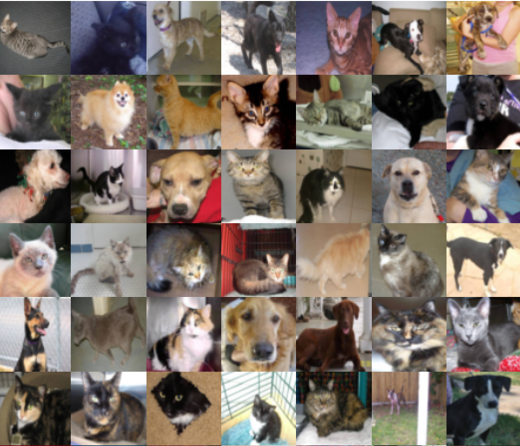
\includegraphics[scale=0.8]{res/catsdogs.png}
\caption[Caption for LOF]{Przykładowe zdjęcia z bazy danych serwisu Kaggle dla konkursu ,,Dogs vs. Cats'' \label{catsdogs}}
\end{figure} 

\subsubsection{Stworzone rozwiązanie}
System stworzony w~przypadku tego eksperymentu składał się z~dwóch głównych komponentów. W~celu wyodrębnienia wczytywania oraz~generowania danych stworzony został komponent nazwany DataProvider, który~pozwalał w~zręczny sposób podawać dane do~sieci. Drugim komponentem była sama sieć neuronowa. Ze~względy jednak na~duże wymogi obliczeniowe w~przypadku uczenia, możliwości dobrania odpowiedniej architektury oraz~optymalizowania parametrów były dość ograniczone. Wszystkie wykorzystywane obrazy zostały zmniejszone do~rozmiarów 64x64. Ostatecznie dobrana architektura sieci zawierała trzy warstwy konwolucyjne, jedną warstwę typu \textit{max pooling}, jedną warstwę w~pełni połączoną  oraz~jedną warstwę wyjściową. Warstwa wyjściowa składała się z~dwóch neuronów odpowiednio dla dwóch rozpoznawanych klas. W~przypadku warstw konwolucyjnych, wszystkie posiadały po~64 filtry z~tym, że~w~pierwszych dwóch stosowana była maska o~rozmiarach 7x7, a~w trzeciej 5x5.  Warstwa w~pełni połączona zawierała 512 neuronów. Obrazy generowane były dynamicznie podczas działania programu. Zastosowane zostały następujące operacje:
\begin{itemize}
\item rotacja obrazu w zakresie od 0 do 40 stopni,
\item przesunięcie w poziomie o długość do 20\% szerokości obrazu,
\item przesunięcie w pionie o długość do 20\% wysokości obrazu,
\item odbicie lustrzane obrazu w poziomie,
\item przybliżenie obrazu do 20\%.
\end{itemize}
Na~rysunku \ref{catdogsimages} został przedstawiony obraz oryginalny oraz~cztery obrazy wygenerowane na~jego podstawie zgodnie z~powyższymi parametrami.

\begin{figure}[ht!]
\centering
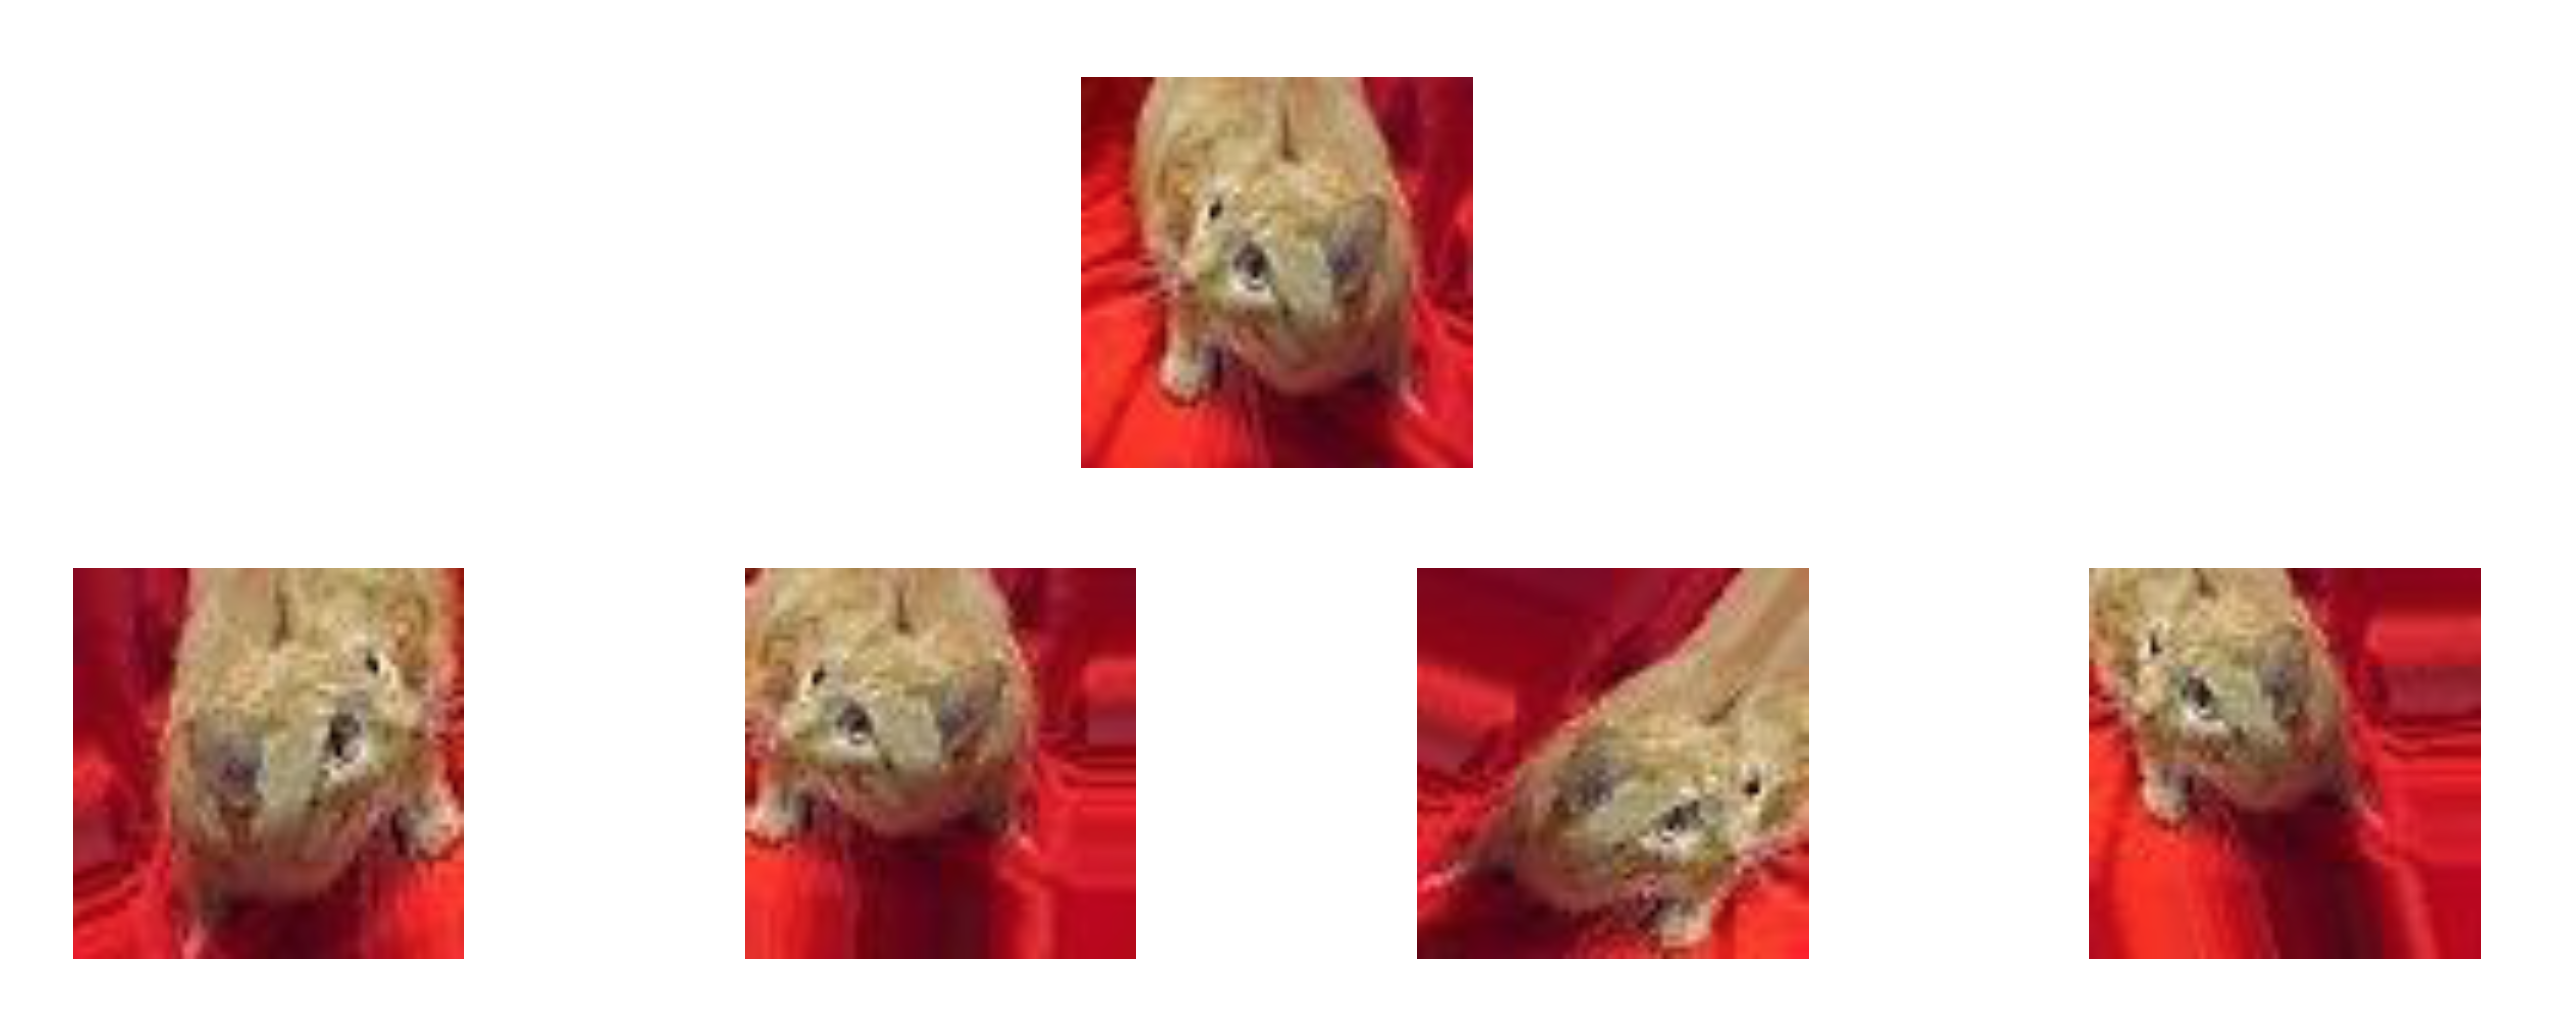
\includegraphics[scale=0.4]{res/catdogsaug.png}
\caption[Caption for LOF]{Obraz oryginalny oraz cztery obrazy wygenerowane na jego podstawie \label{catdogsimages}}
\end{figure} 

\subsubsection{Wyniki}
W~tabeli \ref{table:catdogs} przedstawione zostały wyniki dla sieci uruchamianej przy wykorzystaniu sztucznego powielania cech oraz~bez użycia tej techniki. Na~wykresach \ref{cd_1}, \ref{cd2}, \ref{cd3} przedstawione zostały kolejno skuteczności modelu na~danych testowych w~obu rozważanych przypadkach, skuteczność obliczana na~danych testowych oraz~uczących bez wykorzystania powielania danych, skuteczność obliczana na~danych testowych oraz~uczących przy wykorzystaniu techniki powielania danych.

\begin{table}
\centering
\begin{tabular}{|c|c|}
\hline
Skuteczność uzyskana przy wykorzystaniu sztucznego powielania danych & $72\% \pm 2\%$ \\
\hline 
Skuteczność uzyskana bez wykorzystania sztucznego powielania danych & $69\% \pm 2\%$ \\
\hline 
 \end{tabular}
 \caption{Porównanie wyników z~zastosowaniem metody sztucznego powielania danych} \label{table:catdogs}
\end{table}

\begin{figure}[ht!]
\centering
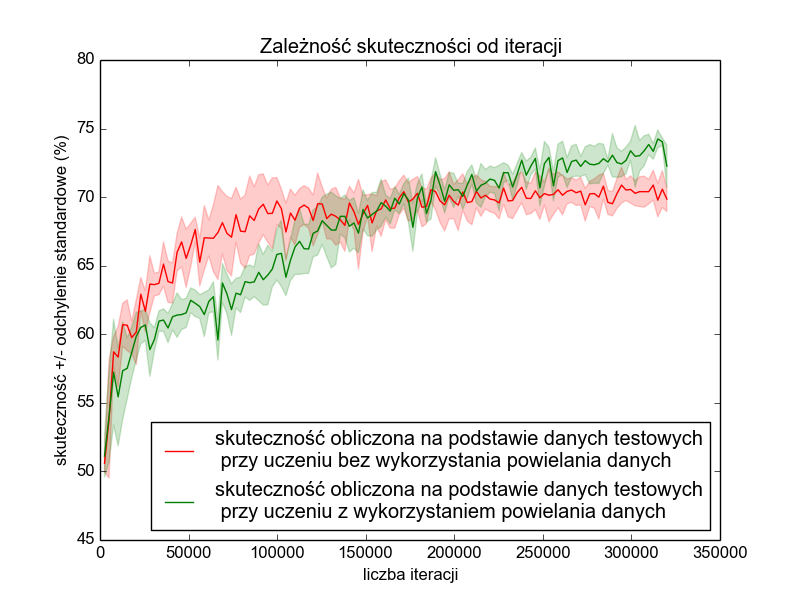
\includegraphics[scale=0.7]{res/comptest.png}
\caption[Caption for LOF]{Porównanie skuteczności w zależności od iteracji obliczana na danych testowych przy uczeniu przy wykorzystaniu powielania danych oraz bez użycia tej techniki\label{cd_1}}
\end{figure} 

\begin{figure}[ht!]
\centering
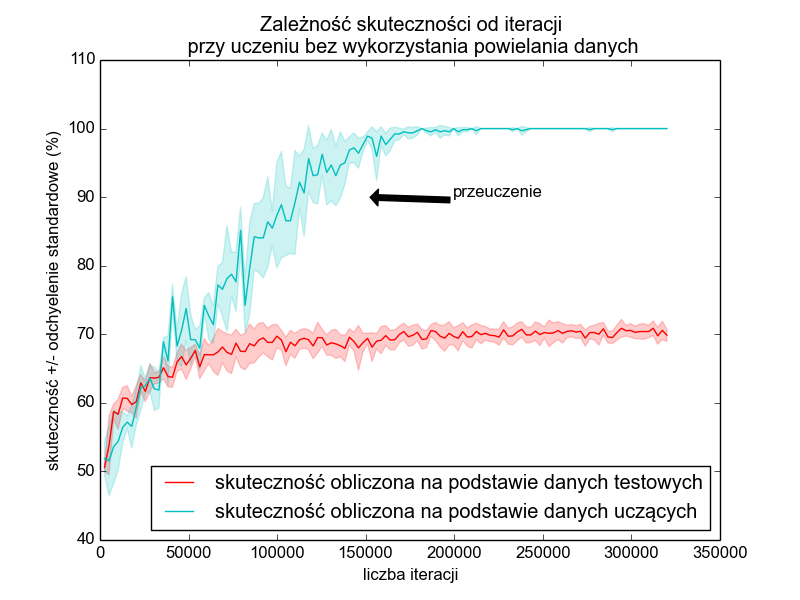
\includegraphics[scale=0.7]{res/testtrain_mulitply.png}
\caption[Caption for LOF]{Porównanie skuteczności w zależności od iteracji obliczana na danych testowych oraz uczących bez wykorzystania powielania danych\label{cd2}}
\end{figure} 

\begin{figure}[ht!]
\centering
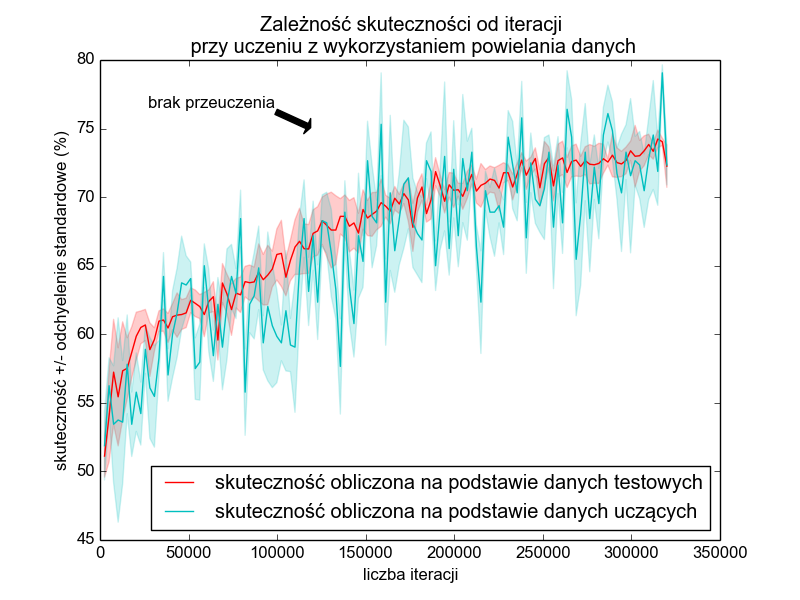
\includegraphics[scale=0.7]{res/testtrain_runtime.png}
\caption[Caption for LOF]{Porównanie skuteczności w zależności od iteracji obliczana na danych testowych oraz uczących z wykorzystania powielania danych\label{cd3}}
\end{figure} 

\subsubsection{Wnioski}
Sztuczne powiększanie zbioru danych, w~analizowanym przypadku nie przyniosło spektakularnej poprawy. Jest to jednak wciąż 2~\%, które~nie kosztuje zbyt wiele. Należy zwrócić uwagę też na~to, iż~w~rzeczywistym przypadku operacja ta może przynieść więcej korzyści pod~warunkiem odpowiedniego doboru jej parametrów, co nie zostało zrobione w~tym przypadku ze~względu na~ograniczone zasoby obliczeniowe. Spoglądając na~rysunek \ref{cd2} łatwo można zauważyć, że~w~przypadku, gdy podawaliśmy do~sieci niezmodyfikowane w~żaden sposób obrazy, szybko doszło do~przeuczenia. Skuteczność obliczana na~podstawie danych uczących osiągnęła 100\% i~sieć nie była w~stanie już więcej nauczyć się na~podstawie danych treningowych. W~przypadku gdy dane zostały sztucznie powielone, możemy zauważyć, na~rysunku \ref{cd3}, że~skuteczność dla zbioru testowego oraz~uczącego oscyluje na~podobnym poziomie w~kolejnych iteracjach. Prawdopodobnie, przeprowadzając uczenie dłużej tj. zwiększając liczbę iteracji, można byłoby spodziewać się, że~różnica w~wyniku przy obu podejściach mogłaby się powiększyć na~korzyść metody z~powielaniem danych, ponieważ~wciąż po~wyznaczonej liczbie iteracji nie doszło do~efektu przeuczenia.

\subsection{Walidacja krzyżowa}\label{cvChapter}
\subsubsection{Opis problemu}
W~tym podrozdziale autor starał się porównać system uczenia maszynowego działający przy zastosowaniu walidacji krzyżowej oraz~tradycyjnego podejścia, w~którym zbiór danych jest dzielony na~zbiór uczący, testowy oraz~walidacyjny. Przeprowadzona została kolejno optymalizacja parametrów dla czterech algorytmów tj. maszyna wektorów nośnych, sztuczne sieci neuronowe, las drzew decyzyjnych oraz~pojedyncze drzewo decyzyjne. Sztuczna sieć neuronowa posiadała jedną warstwę ukrytą. Parametrami optymalizowanymi w~tym przypadku były: liczba neuronów w~warstwie ukrytej oraz~współczynnik uczenia. Dla lasu drzew decyzyjnych optymalizowana była liczba wykorzystanych drzew oraz~ich maksymalna głębokość, natomiast dla drzewa decyzyjnego optymalizowana była tylko maksymalna głębokość drzewa. W~przypadku maszyny wektorów nośnych dobierany był także tylko jeden parametr tj. współczynnik $C$ oraz~wykorzystany był kernel liniowy. W~każdym przypadku optymalizacja parametrów modelu została przeprowadzona za~pomocą metody walidacji krzyżowej oraz~wg tradycyjnego podejścia. Dla każdej pojedynczej optymalizacji następowało uczenie algorytmu 200 razy przed wyborem optymalnych wartości parametrów. W~przypadku wykorzystania walidacji krzyżowej dawało to $10*200$ dla przeprowadzenia optymalizacji. Algorytmy były testowane na~sztucznie wygenerowanych zbiorze zawierającym 7 atrybutów oraz~liczbę rekordów zawierającą się w~zbiorze $ \{200, 500, 1000, 1500, 2000\}.$ Następnie porównane zostały wyniki dla parametrów wyznaczonych wg obu metod dla wszystkich testowanych algorytmów. Należy zwrócić tutaj szczególną uwagę na~fakt, że~optymalizacja przy pomocy walidacji krzyżowej odbywa się na~poziomie doboru odpowiednich parametrów modelu. Po~określeniu parametrów modelu, bez względu na~metodę, którą do~tego wykorzystaliśmy, następuje uczenie oraz~walidacja finalnego modelu. W~przypadku obu podejść, przy uczeniu oraz~walidacji docelowego modelu, użyta zostaje dokładnie taka sama ilość danych. Porównanie użytej ilości danych w~obu przypadkach zostało przedstawione na~rysunku \ref{cvdata}. W~przypadku tradycyjnego podejścia zbiór danych został podzielony na~zbiór uczący stanowiący 60\% wszystkich danych, zbiór testowy stanowiący 20\% wszystkich danych oraz~zbiór walidujący - również 20\% wszystkich danych. W~przypadku walidacji krzyżowej, występowały tylko dwa zbiory tj. zbiór uczący oraz~zbiór walidujący stanowiące kolejno 80\% oraz~20\% wszystkich danych. W~celu uzyskania statystyki, obliczenia dla każdej metody dla konkretnej liczby rekordów powtórzone zostały 10 razy.

\begin{figure}[ht!]
\centering
\includegraphics[scale=0.6]{res/cvdata.png}
\caption[Caption for LOF]{Wykorzystanie danych w zleżności od zastosowanej metody doboru parametrów modelu\label{cvdata}}
\end{figure} 

\subsubsection{Stworzone rozwiązanie}
System stworzony w~celu porównania skuteczności modelu w~zależności od~użytej metody doboru parametrów modelu składał się komponentów takich jak~Main, Optimizer, oraz~Configuration. Pierwszy z~nich odpowiedzialny był za~rozpoczęcie wykonania całej procedury, uwzględniając także wygenerowanie odpowiednich danych. Komponenty nazwane Optimizer oraz~Configuration były kolejno odpowiedzialne za~optymalizację parametrów modelu wg wybranej metody oraz~ogólnej konfiguracji programu, gdzie można wybrać liczbę uruchomień optymalizacji czy~też liczbę rekordów dla których porównanie powinno zostać przeprowadzone. Przeprowadzanie wszystkich założonych obliczeń było bardzo czasochłonne ze~względu na~długość czasu przeprowadzania optymalizacji parametrów modelu, co trwa, w~zależność od~wybranych parametrów, od~kilkudziesięciu minut do~kilku godzin. Biorąc pod~uwagę liczbę możliwości dla tego przykładu, która~jest iloczynem liczby testowanych metod oraz~liczby rekordów dla których przeprowadzane zostały obliczenia, cały proces mógł trwać nawet ponad 40 godzin. W~celu optymalizacji pod~kątem czasu wykonywania programu, obliczenia zostały przeprowadzone z~wykorzystaniem wielowątkowości, co znacznie przyspiesza cały proces, zwłaszcza biorąc uwagę, że~maszyna wykorzystana dla tego zadania posiadała 12 wątków. 
 
\subsubsection{Wyniki}
Zbiorcze wyniki dla wszystkich testowanych wariantów zostały przedstawione w~tabeli \ref{table:cv}. Dla poszczególnych metod uczenia maszynowego, wyniki przedstawione zostały na~rysunkach \ref{cv_ann}, \ref{cv_svm}, \ref{cv_forest}, \ref{cv_tree} kolejno dla sztucznych sieci neuronowych, maszyny wektorów nośnych, lasu drzew decyzyjnych oraz~drzewa decyzyjnego.

% Please add the following required packages to your document preamble:
% \usepackage{multirow}
\begin{table}[]
\centering
\begin{tabular}{|l|l|l|l|l|l|}
\hline
liczba rekordów       & metoda   & ann & forest & svm & tree \\ \hline
\multirow{2}{*}{200}     & holdout    & $ (49,14 \pm 6,2) \% $ & $(45,86 \pm 9,18) \% $ & $(47,71 \pm 5,83) \% $ & $(37,57 \pm 8,48) \% $ \\ \cline{2-6} 
                         & cv         & $(52,14 \pm 5,16) \% $ & $(46,86 \pm 6,79) \% $ & $(48,71 \pm 6,27) \% $ & $(37,63 \pm 7,17) \% $ \\ \hline
\multirow{2}{*}{500}     & holdout    & $(54,4 \pm 5,68) \% $ & $(54,97 \pm 4,98) \% $ & $(50,51 \pm 3,99) \% $ & $(44,74 \pm 3,02) \% $ \\ \cline{2-6} 
                         & cv         & $(59,09 \pm 4,73) \% $ & $(60,34 \pm 3,55) \% $ & $(50,86 \pm 4,4) \% $ & $(45,2 \pm 1,72) \% $ \\ \hline
\multirow{2}{*}{1000}    & holdout    & $(64,11 \pm 3,69) \% $ & $(62,4 \pm 2,89) \% $ & $(56,6 \pm 5,2) \% $ & $(50,4 \pm 3,86) \% $ \\ \cline{2-6} 
                         & cv         & $(64,14 \pm 3,44) \% $ & $(67,51 \pm 4,03) \% $ & $(56,63 \pm 5,26) \% $ & $(49,77 \pm 3,43) \% $ \\\hline
\multirow{2}{*}{1500}    & holdout    &$ (69,24 \pm 2,72) \% $ & $(67,09 \pm 2,66) \% $ & $(58,36 \pm 3,8) \% $ & $(52,69 \pm 2,51) \% $ \\ \cline{2-6} 
                         & cv         & $(69,11 \pm 2,02) \% $ & $(70,97 \pm 1,39) \% $ & $(58,46 \pm 3,79) \% $ & $(52,5 \pm 3,13) \% $ \\ \hline
\multirow{2}{*}{2000}    & holdout    & $(67,74 \pm 4,52) \% $ & $(69,57 \pm 3,5) \% $ & $(58,34 \pm 6,08) \% $ & $(56,44 \pm 3,92) \% $ \\ \cline{2-6} 
                                          & cv         & $(67,74 \pm 4,49) \% $ & $(72,37 \pm 3,01) \% $ & $(58,24 \pm 6,14) \% $ & $(56,71 \pm 3,69) \% $ \\ \hline
                                                                                    
\multicolumn{2}{|l|}{średnia poprawa}   &  $1,52 \%$    &  $3,63 \%$      &  $0,27 \%$   &  $-0,01 \%$   \\ \hline

\end{tabular}
\caption{Skuteczność modelu dla danych walidacyjnych w zależności od testowanego algorytmu uczenia maszynowego oraz wykorzystanej metody optymalizacji parametrów} \label{table:cv}
\end{table}

\newcommand{\cvsize}{1}


\begin{figure}
\centering
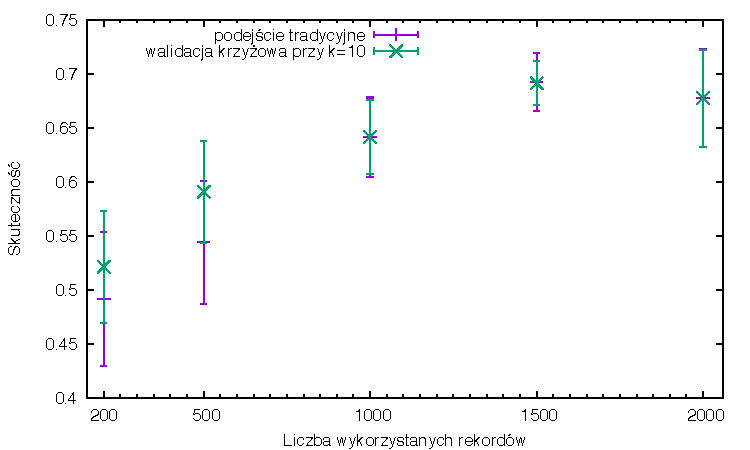
\includegraphics[scale=\cvsize]{res/cv_ann.pdf}
\caption[Caption for LOF]{Porównanie skuteczności modelu przy optymalizacji parametrów przy użyciu walidacji krzyżowej oraz tradycyjnego podejścia dla sztucznych sieci neuronowych\label{cv_ann}}
\end{figure}

\begin{figure}
\centering
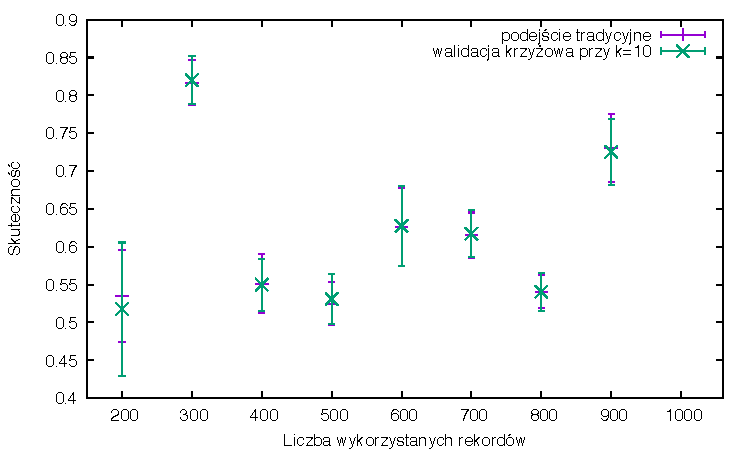
\includegraphics[scale=\cvsize]{res/cv_svm.pdf}
\caption[Caption for LOF]{Porównanie skuteczności modelu przy optymalizacji parametrów przy użyciu walidacji krzyżowej oraz tradycyjnego podejścia dla maszyny wektorów wspierających\label{cv_svm}}
\end{figure}

\begin{figure}
\centering
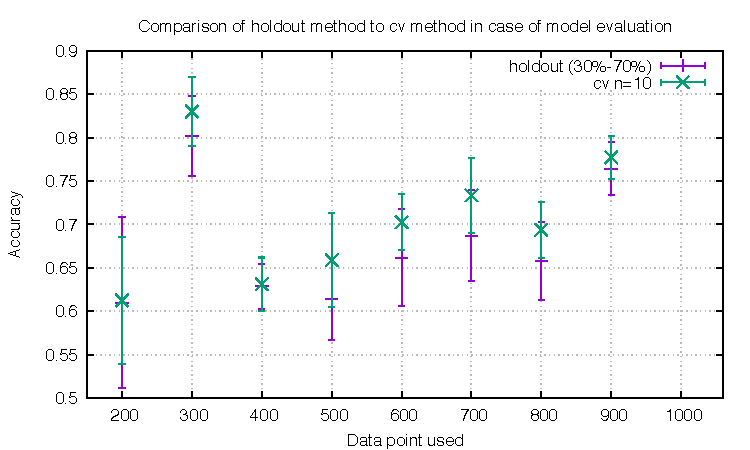
\includegraphics[scale=\cvsize]{res/cv_forest.pdf}
\caption[Caption for LOF]{Porównanie skuteczności modelu przy optymalizacji parametrów przy użyciu walidacji krzyżowej oraz tradycyjnego podejścia dla lasu drzew decyzyjnych\label{cv_forest}}
\end{figure}

\begin{figure}
\centering
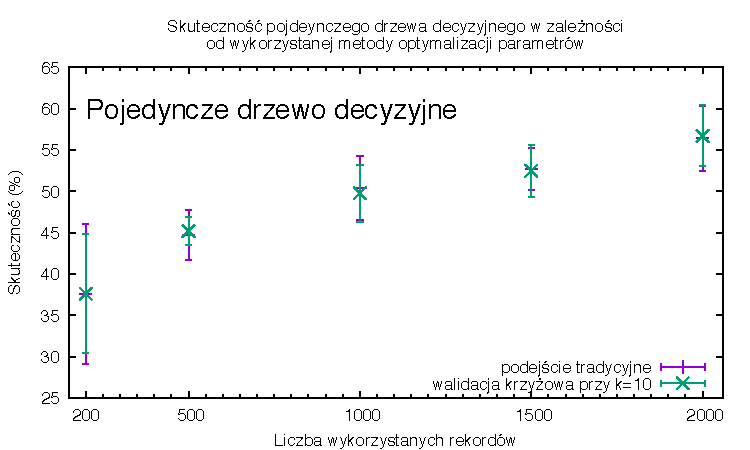
\includegraphics[scale=\cvsize]{res/cv_tree.pdf}
\caption[Caption for LOF]{Porównanie skuteczności modelu przy optymalizacji parametrów przy użyciu walidacji krzyżowej oraz tradycyjnego podejścia dla pojdeynczego drzewa decyzyjnego\label{cv_tree}}
\end{figure}
  


\subsubsection{Wnioski}
Analizując wyniki można stwierdzić, że~poprawa skuteczności klasyfikacji przy użyciu walidacji krzyżowej w~celu wyboru parametrów modelu zależy od~stosowanego algorytmu, a~także od~tego jak~duża liczba rekordów wykorzystana zostaje przy uczeniu algorytmu. Zdecydowanie im więcej rekordów, tym mniejsza poprawa skuteczności. Wynika to z~faktu, iż~powyżej pewnej ilości danych algorytm nie jest w~stanie nauczyć się więcej. Spoglądając na~wykres \ref{cv_ann} możemy zauważyć, że~w~przypadku sieci neuronowych, przy niższej ilości danych, tj. 200 oraz~500 rekordów, poprawa wynosi aż kilka procent, co jest bardzo zadowalającym wynikiem. W~przypadku większej liczby rekordów wynik jest porównywalny bez względu na~wykorzystaną metodę optymalizacji. W~przypadku drzewa decyzyjnego oraz~maszyny wektorów wspierających wartość skuteczności nie różni się na~tyle, aby~mówić o~jakiejkolwiek zmianie bez względu na~użytą metodę doboru parametrów, co może wynikać z~faktu, iż~w~przypadku obu tych metod tylko jeden parametr był optymalizowany (w przypadku sieci neuronowyh oraz~lasu drzew decyzyjnych były optymalizowane 2 parametry). Wpływ optymalizacji na~skuteczność jest mniejszy w~takim przypadku. Zwiększyć można byłoby go poprzez~rozszerzenie zakresu optymalizacji.

\subsection{Ekstrakcja cech przy użyciu metod matematycznych}

\subsubsection{Opis problemu}
Metodę wykorzystaną w~celu ekstrakcji cech w~ramach metod matematycznych była liniowa analiza dyskryminacyjna. Przetestowane zostały cztery algorytmy uczenia maszynowego tj. maszyna wektorów nośnych, sztuczne sieci neuronowe, las drzew decyzyjnych oraz~pojedyncze drzewo decyzyjne. Wykorzystanym zbiorem danych był zbiór o~nazwie \textit{iris} dostępny w~bibliotece Scikit-Learn\footnote{\url{http://scikit-learn.org/stable/auto_examples/datasets/plot_iris_dataset.html}}. Posiada on 4 atrybuty, które~mówią o~rozmiarach irysów 3 różnych gatunków, a~więc, co za~tym idzie, cały zbiór podzielony jest na~3 klasy. Każdy rekord zbioru reprezentuje kwiat. Zbiór zawiera 150 rekordów, po~50 dla każdej gatunku. Zbiór ten był wprowadzony przez~brytyjskiego statystyka oraz~biologa Ronalda Fishera, którego~rola była znacząca w~rozwoju statystyki. Eksperyment polegał na~kolejno:
\begin{itemize}

\item przeprowadzeniu optymalizacji parametrów modeli dla poszczególnych metod,
\item uczeniu oraz testowaniu systemu.

\end{itemize}

Powyższe kroki wykonane zostały w~zależności od~liczby rekordów oraz~liczby atrybutów zbioru. Liczba rekordów dla których przeprowadzone zostały testy mieściła się w~zbiorze $ \{10, 20, 30, 40, 50, 100\} $. Obliczenia przeprowadzone zostały dla liczby atrybutów początkowo wynoszącej 4, 2 oraz~1. Celem było określenie czy, oraz~na~ile, ekstrakcja cech może pomóc w~otrzymaniu wyższej skuteczności przy uczeniu maszynowym. Wszystkie obliczenia wykonane zostały w~każdym przypadku 10 razy w~celu uzyskania odpowiedniej statystyki wyników.

\subsubsection{Stworzone rozwiązanie}
Stworzony system składał się z~komponentów takich jak~Main, Optimizer oraz~Configuration. Podobnie jak~w~eksperymencie opisanym w~podrozdziale \ref{cvChapter} były odpowiedzialne kolejno za~zadania uruchomienia głównego programu, optymalizacji parametrów modelu oraz~konfigurację. Dodatkowo, w~komponencie Main, znajduję się logika programu odpowiedzialna za~redukcję wymiarowości zbioru danych. Także i~w tym przypadku wykonywanie całej procedury dla różnych przypadków trwało dość długo tj. od~kilku do~kilkunastu godzin, co stanowiło motywację do~wykorzystania wielowątkowości.

\subsubsection{Wyniki}
Zbiorcze wyniki dla różnej ilości wykorzystanych danych zostały przedstawione w~tabeli \ref{table:fxTable} oraz~na~rysunku \ref{extractionSummary}. Dodatkowo, na~rysunku \ref{showMeIris} przedstawiony został zbiór danych \textit{iris} pod~redukcji do~dwóch wymiarów oraz~do~jednego wymiaru.


\begin{figure}[ht!]
\centering
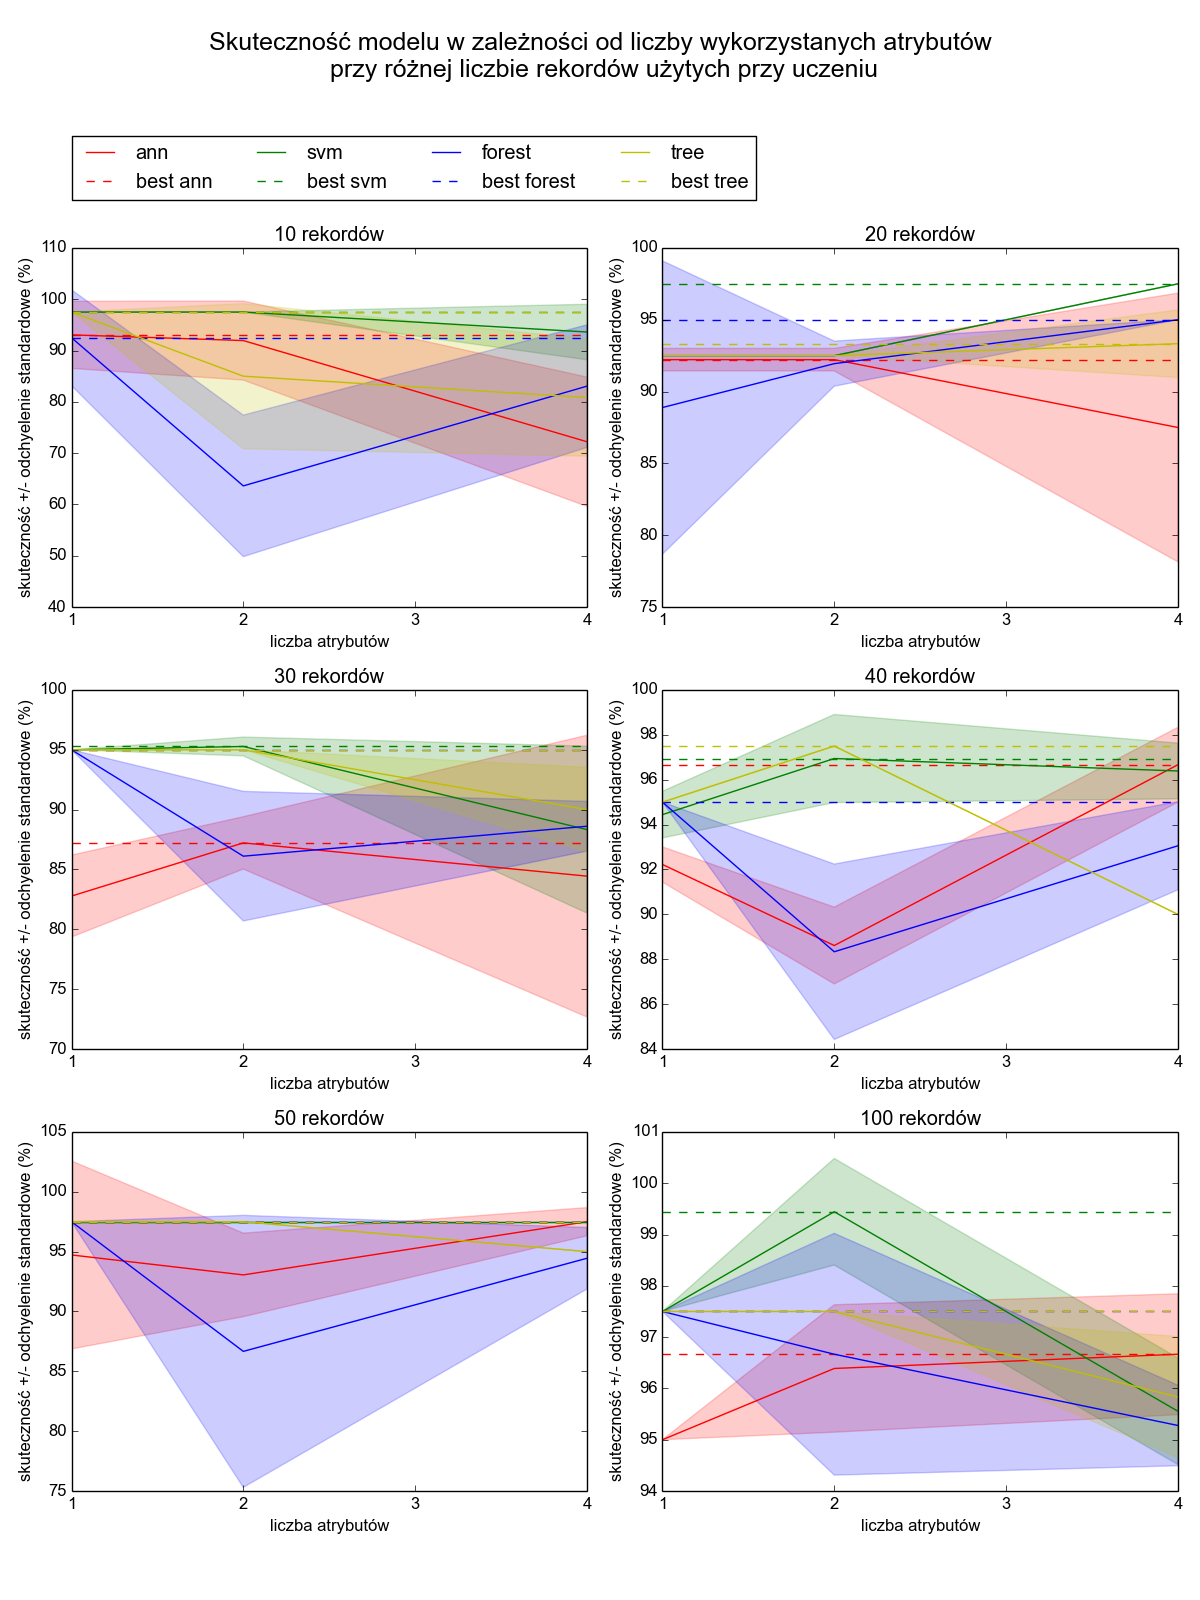
\includegraphics[scale=0.45]{res/extractionSummary.png}
\caption[Caption for LOF]{Porwóananie skuteczności modelu dla różnych algorytmów w zależności od liczby atrybutów oraz ilości wykorzystanych do uczenia danych\label{extractionSummary}}
\end{figure} 

\begin{figure}[ht!]
\centering
\includegraphics[scale=0.45]{res/showMeIris.png}
\caption[Caption for LOF]{Zbiór danych \textit{iris} po przeprowadzeniu ekstrakcji cech\label{showMeIris}}
\end{figure} 

% Please add the following required packages to your document preamble:
% \usepackage{multirow}
\begin{table}[]
\tiny
\centering
\begin{tabular}{|c|c|c|c|c|}
\hline
Liczba rekordów       & Metoda                  & Liczba atrybutów & Skuteczność & Poprawa \\ \hline
\multirow{12}{*}{10}  & \multirow{3}{*}{ann}    & 1                & $ (93,06  \pm  6,54) \% $ & \multirow{3}{*}{$20,84\%$} \\ \cline{3-4} 
                      &                         & 2                & $ (91,94 \pm 7,71) \% $   & \\ \cline{3-4} 
                      &                         & 4                & $ (72,22 \pm 12,61) \% $  & \\ \cline{2-5} 
                      & \multirow{3}{*}{svm}    & 1                & $ (97,5 \pm 0) \% $        & \multirow{3}{*}{$3,89 \%$} \\ \cline{3-4} 
                      &                         & 2                & $ (97,5 \pm 0) \% $       &\\ \cline{3-4} 
                      &                         & 4                & $ (93,61 \pm 5,41) \% $   &\\ \cline{2-5} 
                      & \multirow{3}{*}{forest} & 1                & $ (92,5 \pm 9,35) \% $    & \multirow{3}{*}{$9,44\%$} \\ \cline{3-4} 
                      &                         & 2                & $ (63,61 \pm 13,8) \% $   &\\ \cline{3-4} 
                      &                         & 4                & $ (83,06 \pm 11,95) \% $ & \\ \cline{2-5} 
                      & \multirow{3}{*}{tree}   & 1                & $ (97,5 \pm 0) \% $       & \multirow{3}{*}{$16,67\%$} \\ \cline{3-4} 
                      &                         & 2                & $ (85 \pm  14,14) \% $    & \\ \cline{3-4} 
                      &                         & 4                & $ (80,83 \pm 11,43) \% $  &\\ \hline
\multirow{12}{*}{20}  & \multirow{3}{*}{ann}    & 1                & $ (92,22 \pm 0,79) \% $   & \multirow{3}{*}{$4,72\%$} \\ \cline{3-4} 
                      &                         & 2                & $ (92,22 \pm 0,79) \% $   &\\ \cline{3-4} 
                      &                         & 4                & $ (87,5 \pm 9,35) \% $    &\\ \cline{2-5} 
                      & \multirow{3}{*}{svm}    & 1                & $ (92,5 \pm 0) \% $       & \multirow{3}{*}{$-5 \%$} \\ \cline{3-4} 
                      &                         & 2                & $ (92,5 \pm 0) \% $       &\\ \cline{3-4} 
                      &                         & 4                & $ (97,5 \pm 0) \% $       &\\ \cline{2-5} 
                      & \multirow{3}{*}{forest} & 1                & $ (88,89 \pm 10,21) \% $  & \multirow{3}{*}{$-3,06 \%$} \\ \cline{3-4} 
                      &                         & 2                & $ (91,94 \pm 1,57) \% $  & \\ \cline{3-4} 
                      &                         & 4                & $ (95 \pm 0) \% $         &\\ \cline{2-5} 
                      & \multirow{3}{*}{tree}   & 1                & $ (92,5 \pm 0) \% $       & \multirow{3}{*}{$-0,83 \%$} \\ \cline{3-4} 
                      &                         & 2                & $ (92,5 \pm 0) \% $       &\\ \cline{3-4} 
                      &                         & 4                & $ (93,33 \pm 2,36) \% $   &\\ \hline
\multirow{12}{*}{30}  & \multirow{3}{*}{ann}    & 1                & $ (82,78 \pm 3,42) \% $   & \multirow{3}{*}{$2,78\%$} \\ \cline{3-4} 
                      &                         & 2                & $ (87,22 \pm 2,19) \% $  & \\ \cline{3-4} 
                      &                         & 4                & $ (84,44 \pm 11,77) \% $  &\\ \cline{2-5} 
                      & \multirow{3}{*}{svm}    & 1                & $ (95 \pm 0) \% $        & \multirow{3}{*}{$6,95\%$} \\ \cline{3-4} 
                      &                         & 2                & $ (95,28 \pm 0,79) \% $   &\\ \cline{3-4} 
                      &                         & 4                & $ (88,33 \pm 6,97) \% $   &\\ \cline{2-5} 
                      & \multirow{3}{*}{forest} & 1                & $ (95 \pm 0) \%  $        & \multirow{3}{*}{$6,39\%$} \\ \cline{3-4} 
                      &                         & 2                & $ (86,11 \pm 5,41) \% $   &\\ \cline{3-4} 
                      &                         & 4                & $ (88,61 \pm 2,08) \% $  & \\ \cline{2-5} 
                      & \multirow{3}{*}{tree}   & 1                & $ (95 \pm 0) \%  $       & \multirow{3}{*}{$5\%$} \\ \cline{3-4} 
                      &                         & 2                & $ (95 \pm 0) \%  $       &\\ \cline{3-4} 
                      &                         & 4                & $ (90 \pm  3,54) \% $     & \\ \hline
\multirow{12}{*}{40}  & \multirow{3}{*}{ann}    & 1                & $ (92,22 \pm 0,79) \% $   & \multirow{3}{*}{$-4,55  \%$} \\ \cline{3-4} 
                      &                         & 2                & $ (88,61 \pm 1,71) \% $   &\\ \cline{3-4} 
                      &                         & 4                & $ (96,67 \pm 1,67) \% $  & \\ \cline{2-5} 
                      & \multirow{3}{*}{svm}    & 1                & $ (94,44 \pm 1,04) \% $   & \multirow{3}{*}{$0,55$\%} \\ \cline{3-4} 
                      &                         & 2                & $ (96,94 \pm 1,96) \% $  & \\ \cline{3-4} 
                      &                         & 4                & $ (96,39 \pm 1,24) \% $   &\\ \cline{2-5} 
                      & \multirow{3}{*}{forest} & 1                & $ (95 \pm 0) \% $        & \multirow{3}{*}{$1,94$\%} \\ \cline{3-4} 
                      &                         & 2                & $ (88,33 \pm 3,91) \% $   &\\ \cline{3-4} 
                      &                         & 4                & $ (93,06 \pm 1,96) \% $   &\\ \cline{2-5} 
                      & \multirow{3}{*}{tree}   & 1                & $ (95 \pm 0) \% $         & \multirow{3}{*}{$7,5\%$} \\ \cline{3-4} 
                      &                         & 2                & $ (97,5 \pm 0) \% $      &\\ \cline{3-4} 
                      &                         & 4                & $ (90 \pm 0) \%   $     & \\ \hline
\multirow{12}{*}{50}  & \multirow{3}{*}{ann}    & 1                & $ (94,72 \pm 7,86) \% $   & \multirow{3}{*}{$-2,78 \%$} \\ \cline{3-4} 
                      &                         & 2                & $ (93,06 \pm 3,49) \% $  & \\ \cline{3-4} 
                      &                         & 4                & $ (97,5 \pm 1,18) \% $    &\\ \cline{2-5} 
                      & \multirow{3}{*}{svm}    & 1                & $ (97,5 \pm 0) \% $       & \multirow{3}{*}{$0 \%$} \\ \cline{3-4} 
                      &                         & 2                & $ (97,5 \pm 0) \% $     &  \\ \cline{3-4} 
                      &                         & 4                & $ (97,5 \pm 0) \% $       & \\ \cline{2-5} 
                      & \multirow{3}{*}{forest} & 1                & $ (97,5 \pm 0) \% $       & \multirow{3}{*}{$3.06\%$} \\ \cline{3-4} 
                      &                         & 2                & $ (86,67 \pm 11,37) \% $ & \\ \cline{3-4} 
                      &                         & 4                & $ (94,44 \pm 2,58) \% $   &\\ \cline{2-5} 
                      & \multirow{3}{*}{tree}   & 1                & $ (97,5 \pm 0) \% $       & \multirow{3}{*}{$2.5\%$} \\ \cline{3-4} 
                      &                         & 2                & $ (97,5 \pm 0) \% $      & \\ \cline{3-4} 
                      &                         & 4                & $ (95 \pm 0) \%   $      &\\ \hline
\multirow{12}{*}{100} & \multirow{3}{*}{ann}    & 1                & $ (95 \pm 0) \%   $      & \multirow{3}{*}{$-1,67 \%$} \\ \cline{3-4} 
                      &                         & 2                & $ (96,39 \pm 1,24) \% $   &\\ \cline{3-4} 
                      &                         & 4                & $ (96,67 \pm 1,18) \% $  & \\ \cline{2-5} 
                      & \multirow{3}{*}{svm}    & 1                & $ (97,5 \pm 0) \% $       & \multirow{3}{*}{$3,88\%$} \\ \cline{3-4} 
                      &                         & 2                & $ (99,44 \pm 1,04) \% $  & \\ \cline{3-4} 
                      &                         & 4                & $ (95,56 \pm 1,04) \% $  & \\ \cline{2-5} 
                      & \multirow{3}{*}{forest} & 1                & $ (97,5 \pm 0) \% $       & \multirow{3}{*}{$2,22\%$} \\ \cline{3-4} 
                      &                         & 2                & $ (96,67 \pm 2,36) \% $   &\\ \cline{3-4} 
                      &                         & 4                & $ (95,28 \pm 0,79) \% $  & \\ \cline{2-5} 
                      & \multirow{3}{*}{tree}   & 1                & $ (97,5 \pm 0) \% $       & \multirow{3}{*}{$1,67\%$} \\ \cline{3-4} 
                      &                         & 2                & $ (97,5 \pm 0) \% $       &\\ \cline{3-4} 
                      &                         & 4                & $ (95,83 \pm 1,18) \% $   &\\ \hline
\end{tabular}
\caption{Zestawienie skuteczności przy wykorzystaniu ekstrakcji cech przy użyciu różnej liczby rekordów, różne liczby atrybutów w zależności od wybranej metody}
\label{table:fxTable}

\end{table}

\subsubsection{Wnioski}
Analizując jako pierwszy wykres na~rysunku \ref{showMeIris}, można zauważyć, że~dane ze~zbioru \textit{iris} są prawie separowalne liniowo. Stwarza to możliwość efektywnego wykorzystania metody LDA w~celu ekstrakcji cech. Trzeba jednak pamiętać, że~tego typu zbiory raczej nie są zbyt często spotykane w~rzeczywistości. Wykres przedstawiający opracowywane dane w~jednym wymiarze pokazuje, że~transformacja do~takiej przestrzeni nie stanowi wciąż problemu jeśli chodzi o~realizację zadania klasyfikacji w~tym przypadku. Posiadanie danych o~mniejszej ilości atrybutów pozwala użyć prostszych modeli, co z~kolei przeciwdziała przeuczeniu, które~jest znacznym problemem w~przypadku niskiej ilości danych. W~przypadku posiadania tylko 10 rekordów w~celu przeprowadzenia uczenia, można zauważyć jak~bardzo pomocna okazuje się tutaj ekstrakcja cech. Poprawa skuteczności została odnotowana dla wszystkich metod i~to bardzo w~znacznym stopniu w~przypadku algorytmu drzewa decyzyjnego oraz~sztucznych sieci neuronowych, bo~aż $16,67 \%$ w~pierwszym oraz~$20,84 \%$ przypadku drugim (patrz tabela \ref{table:fxTable}). Dla lasu drzew decyzyjnych oraz~maszyny wektorów wspierających poprawa wynosiła kolejno $9,44 \%$ oraz~$3,89 \%$, co wciąż jest zadowalającym wynikiem.  Należy jednak zwrócić jednak na~odchylenie standardowe. Jego wysoka wartość oznacza duże fluktuacje. Z~reguły im mniej danych było wykorzystywanych, tym większa wartość odchylenia standardowego była odnotowywana. Jest to naturalne zjawisko. Im mniej danych, tym wynik jest bardziej przypadkowy ze~względu na~fakt, iż~dane uczące są losowo wybierane z~całego zbioru. W~niektórych przypadkach można też zauważyć bardzo niewielką zmianą albo~też nawet całkowity jej brak jeśli chodzi o~wynik oraz~odchylenie standardowe (np. SVM dla 50 rekordów). Jest to również pozytywne zjawisko. Korzystając z~danych o~mniejszej liczbie wymiarów udało się osiągnąć ten sam efekt, co oznacza, że~mniej obliczeń zostało przeprowadzonych, a~skuteczność oraz~odchylenie standardowe pozostały na~podobnym poziomie. Przy większej ilości danych, poprawa skuteczności nie zawsze występowała, ale~wciąż w~większości przypadków wyniki uzyskiwane po~przeprowadzeniu ekstrakcji były lepsze (poprawa została odnotowana w~13 na~20 pozostałych przypadków). Podsumowując, ekstrakcja cech stanowi bardzo dobry sposób na~optymalizację uczenia maszynowego pod~kątem ilości danych, lecz wydaje się, że~nie może być bardzo często stosowana ze~względu na~wymóg liniowej separowalność danych. Istnieją jednakże algorytmy, które~są w~stanie przeprowadzić ekstrakcję danych, które~nie są separowalne liniowo. Sama sieć neuronowa może zostać wykorzystana w~celu nielinowej ekstrakcji cech.  Podejście to zostało opisane w~pracy \cite{bishop1995neural} (strona 314).

\subsection{Ekstrakcja cech przy użyciu ,,wiedzy''}
\subsubsection{Opis problemu}
W~niniejszym podrozdziale rozważanym zagadnieniem była ekstrakcja cech przy użyciu ,,wiedzy'', która~polega na~transformacji danych do~przestrzeni o~mniejszej wymiarowości przy wykorzystaniu wiedzy, którą posiadamy na~temat naszych danych. Pomysł na~ten eksperyment został zaczerpnięty z~pracy~\cite{higgs1}. Wykorzystane zostały także dane opisane w~artykule, które~są danymi symulowanymi mającymi posłużyć jako podstawa dla stworzenia modelu, który~jest w~stanie odróżnić tło od~sygnału przy czym w~tym przypadku sygnałem jest bozon Higgsa, którego~istnienie zostało potwierdzone w~2013 roku. 
Badania dotyczące fizyki cząstek przeprowadzane sa  w~Europejskim Ośrodku Badań Jądrowych CERN w~pobliżu Genewy. Najbardziej spektakularnym narzędziem do~tego wykorzystywanym jest Wielki Zderzacz Hadronów (\textit{Large Hadron Collider}, LHC), który~jest największym na~świecie akceleratorem cząstek na~świecie. W~celu izolacji sygnału od~tła, w~przypadku danych z~odpowiednich detektorów cząstek, szeroko wykorzystywane jest uczenie maszynowe. Artykuł opisuje wykorzystanie głębokich sieci neuronowych dla problemu wyodrębnienia cząstki Higgsa. Udostępnione dane zawierają 11 milionów rekordów dla których określonych jest 21 cech fizycznych tzw. niskiego poziomu. Każdy rekord opisany jest także za~pomocą 7 atrybutów wysokiego poziomu, które~obliczone zostały na~podstawie cech niskiego poziomu. Celem obliczeń było pokazanie, że~poniżej pewnej ilości danych, użycie niskiego poziomu daje gorsze wyniki niż wykorzystanie cech wysokiego poziomu. Ekstrakcja cech przy użyciu ,,wiedzy'' można więc traktować jako optymalizację pod~kątem niskiej ilości danych. Obok głębokiej sieci neuronowej, wykorzystane zostały algorytmy takie jak~tradycyjne sieć neuronowa, las drzew decyzyjnych oraz~pojedyncze drzewo decyzyjne. Dla wszystkich wymienionych tradycyjnych algorytmów uczenia maszynowego przeprowadzona została optymalizacja parametrów. W~przypadku głębokiej sieci neuronowej nie miało to miejsca ze~względu na~bardzo długi czas uczenia. W~przypadku wszystkich metod obliczenia przeprowadzone zostały dla cech wysokiego oraz~niskiego poziomu, a~także dla różnej ilości danych, które~były fragmentami całego udostępnionego zbioru. Rozważone zostały ułamki $a$ całego zbioru przy czym $a\in\{0,001; 0,005; 0,01; 0,05; 0,1; 0,2; 0,3; 0,4; 0,5\}$. 

\subsubsection{Stworzone rozwiązanie}
Stworzony system składał się z~trzech elementów z~których można wyróżnić: HiggsModel, Optimizer oraz~Configuration. Były odpowiedzialne kolejno za~tworzenie głębokie sieci neuronowej (oparty na~pracy \cite{higgs2}), optymalizację parametrów dla poszczególnych algorytmów oraz~konfiguracji programu. W~przypadku głębokiej sieci neuronowej, wykorzystana została sieć posiadająca 6 warstw ukrytych po~500 neuronów w~każdej. Podobnie jak~w~przypadków poprzednich obliczeń, autor skorzystał z~dobrodziejstw wielowątkowości w~celu ich przyspieszenia.


\subsubsection{Wyniki}
Na~rysunkach \ref{higgsall1} oraz~\ref{higgsall2} przedstawione została krzywa ROC dla $a\in\{0,001; 0,005; 0,01; 0,05; 0,1\}$  oraz~dla $a\in\{0,2; 0,3; 0,4; 0,5\}$. AUC ROC dla wszystkich testowanych kombinacji zostało przedstawione w~tabeli \ref{table:higgstable} oraz~przedstawione na~rysunku \ref{higgssummary}.


% Please add the following required packages to your document preamble:
% \usepackage{multirow}
\begin{table}[]
\centering
\begin{tabular}{|c|c|c|c|c|c|}
\hline
\multirow{2}{*}{a}                      &  \multirow{2}{*}{wykorzystane cechy} & \multicolumn{4}{c|}{AUC ROC} \\ \cline{3-6}

 &       & tree & forest & ann & dnn \\ \hline

\multirow{2}{*}{0,001} & niskiego poziomu   & $ 0,6 $ & $ 0,62 $ & $ 0,62 $ &$ 0,62 $ \\ \cline{2-6} 
                       & wysokiego poziomu & $ 0,71 $ & $ 0,77 $ & $ 0,66 $ &$ 0,72 $ \\ \hline 
                       
\multirow{2}{*}{0,005} & niskiego poziomu  & $ 0,63 $ & $ 0,63 $ & $ 0,63 $ &$ 0,67 $ \\ \cline{2-6} 
                       & wysokiego poziomu & $ 0,74 $ & $ 0,75 $ & $ 0,69 $ &$ 0,77 $ \\ \hline
                       
\multirow{2}{*}{0,01}  & niskiego poziomu  & $ 0,64 $ & $ 0,64 $ & $ 0,63 $ &$ 0,7 $ \\ \cline{2-6} 
                       & wysokiego poziomu & $ 0,74 $ & $ 0,75 $ & $ 0,7 $ &$ 0,77 $ \\ \hline
                       
\multirow{2}{*}{0,05}  & niskiego poziomu  & $ 0,66 $ & $ 0,64 $ & $ 0,64 $ &$ 0,76 $ \\ \cline{2-6} 
                       & wysokiego poziomu &  $ 0,75 $ & $ 0,74 $ & $ 0,7 $ &$ 0,78 $ \\ \hline
                       
\multirow{2}{*}{0,1}   & niskiego poziomu  &  $ 0,66 $ & $ 0,64 $ & $ 0,64 $ &$ 0,79 $ \\ \cline{2-6} 
                       & wysokiego poziomu &  $ 0,76 $ & $ 0,74 $ & $ 0,7 $ &$ 0,79 $ \\ \hline
                       
\multirow{2}{*}{0,2}   & niskiego poziomu  &  $ 0,67 $ & $ 0,64 $ & $ 0,64 $ &$ 0,81 $ \\ \cline{2-6} 
                       & wysokiego poziomu &  $ 0,77 $ & $ 0,74 $ & $ 0,7 $ &$ 0,79 $ \\ \hline
                       
\multirow{2}{*}{0,3}   & niskiego poziomu  &  $ 0,67 $ & $ 0,64 $ & $ 0,64 $ &$ 0,82 $ \\ \cline{2-6} 
                       & wysokiego poziomu &  $ 0,77 $ & $ 0,74 $ & $ 0,7 $ &$ 0,79 $ \\ \hline
                       
\multirow{2}{*}{0,4}   & niskiego poziomu  & $ 0,67 $ & $ 0,64 $ & $ 0,65 $ &$ 0,83 $ \\ \cline{2-6} 
                       & wysokiego poziomu &  $ 0,77 $ & $ 0,74 $ & $ 0,7 $ &$ 0,79 $ \\ \hline
                       
\multirow{2}{*}{0,5}   & niskiego poziomu  &  $ 0,68 $ & $ 0,64 $ & $ 0,64 $ &$ 0,83 $ \\ \cline{2-6} 
                       & wysokiego poziomu &  $ 0,77 $ & $ 0,74 $ & $ 0,69 $ &$ 0,79 $ \\ \hline
\end{tabular}

\caption{Zestawienie AUC ROC dla testowanych metod w zależności od rodzaju wykorzystanych cech oraz ilości wykorzystanych danych}
\label{table:higgstable}

\end{table}


\begin{figure}[ht!]
\centering
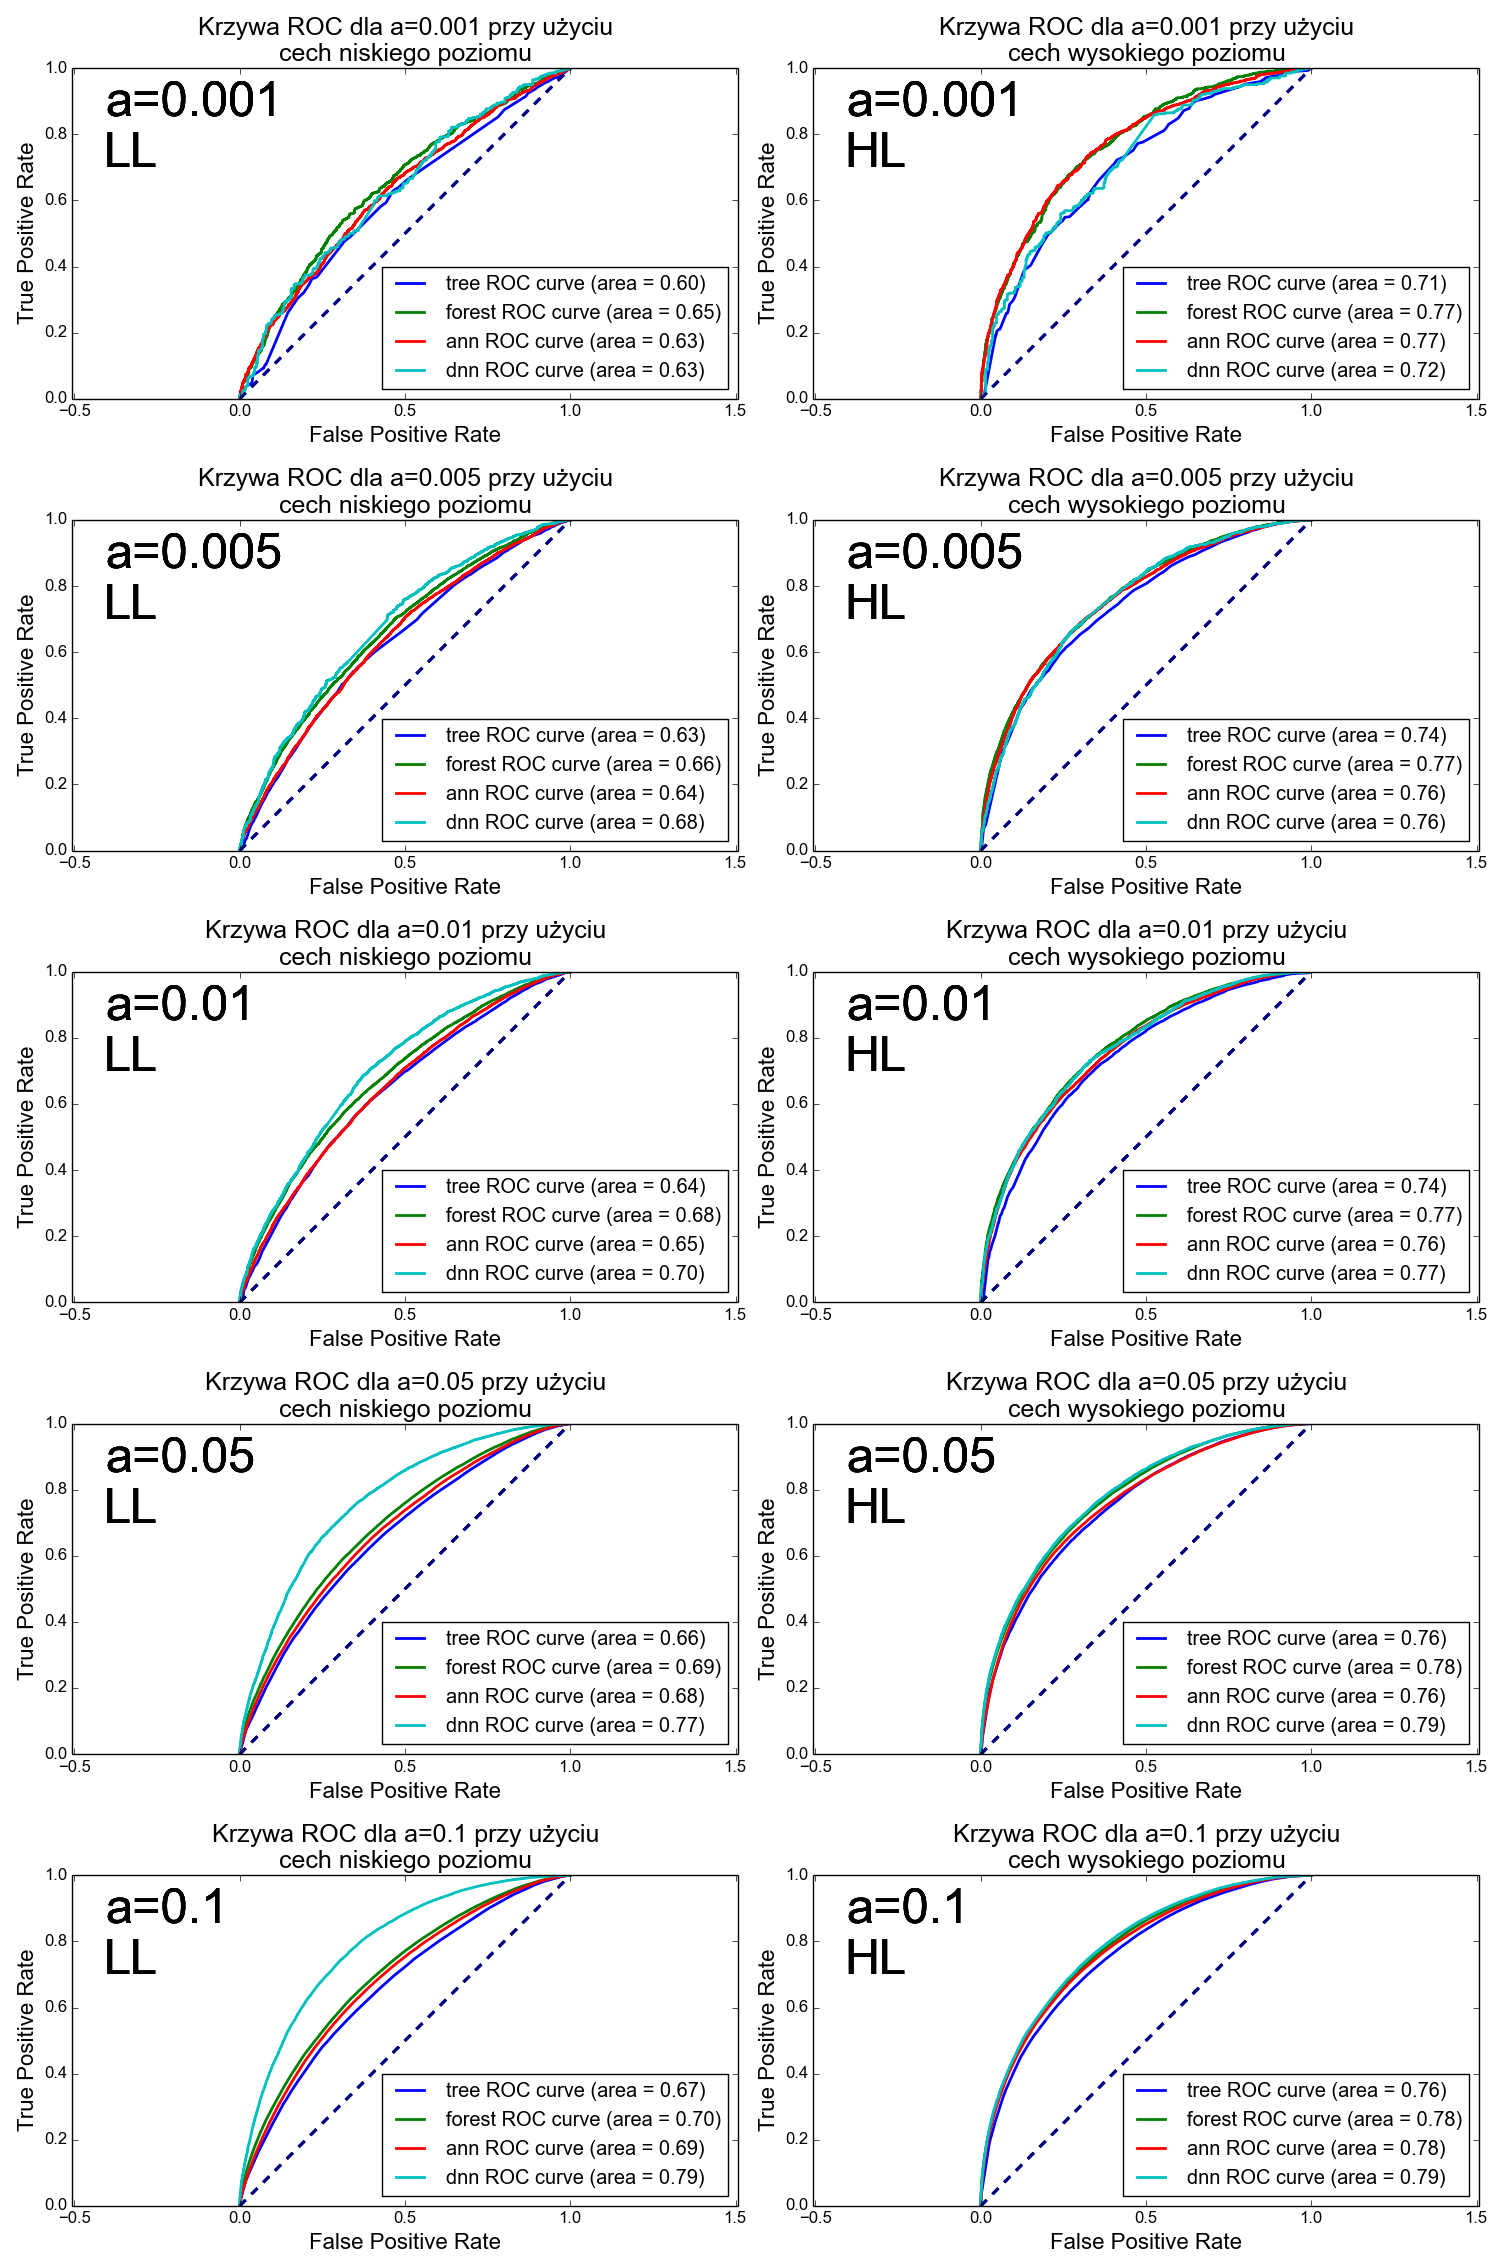
\includegraphics[scale=0.425]{res/allnew1.png}
\caption[Caption for LOF]{Krzywa ROC dla $a\in\{0.001, 0.005, 0.01, 0.05, 0.1\}$\label{higgsall1}}
\end{figure} 

\begin{figure}[ht!]
\centering
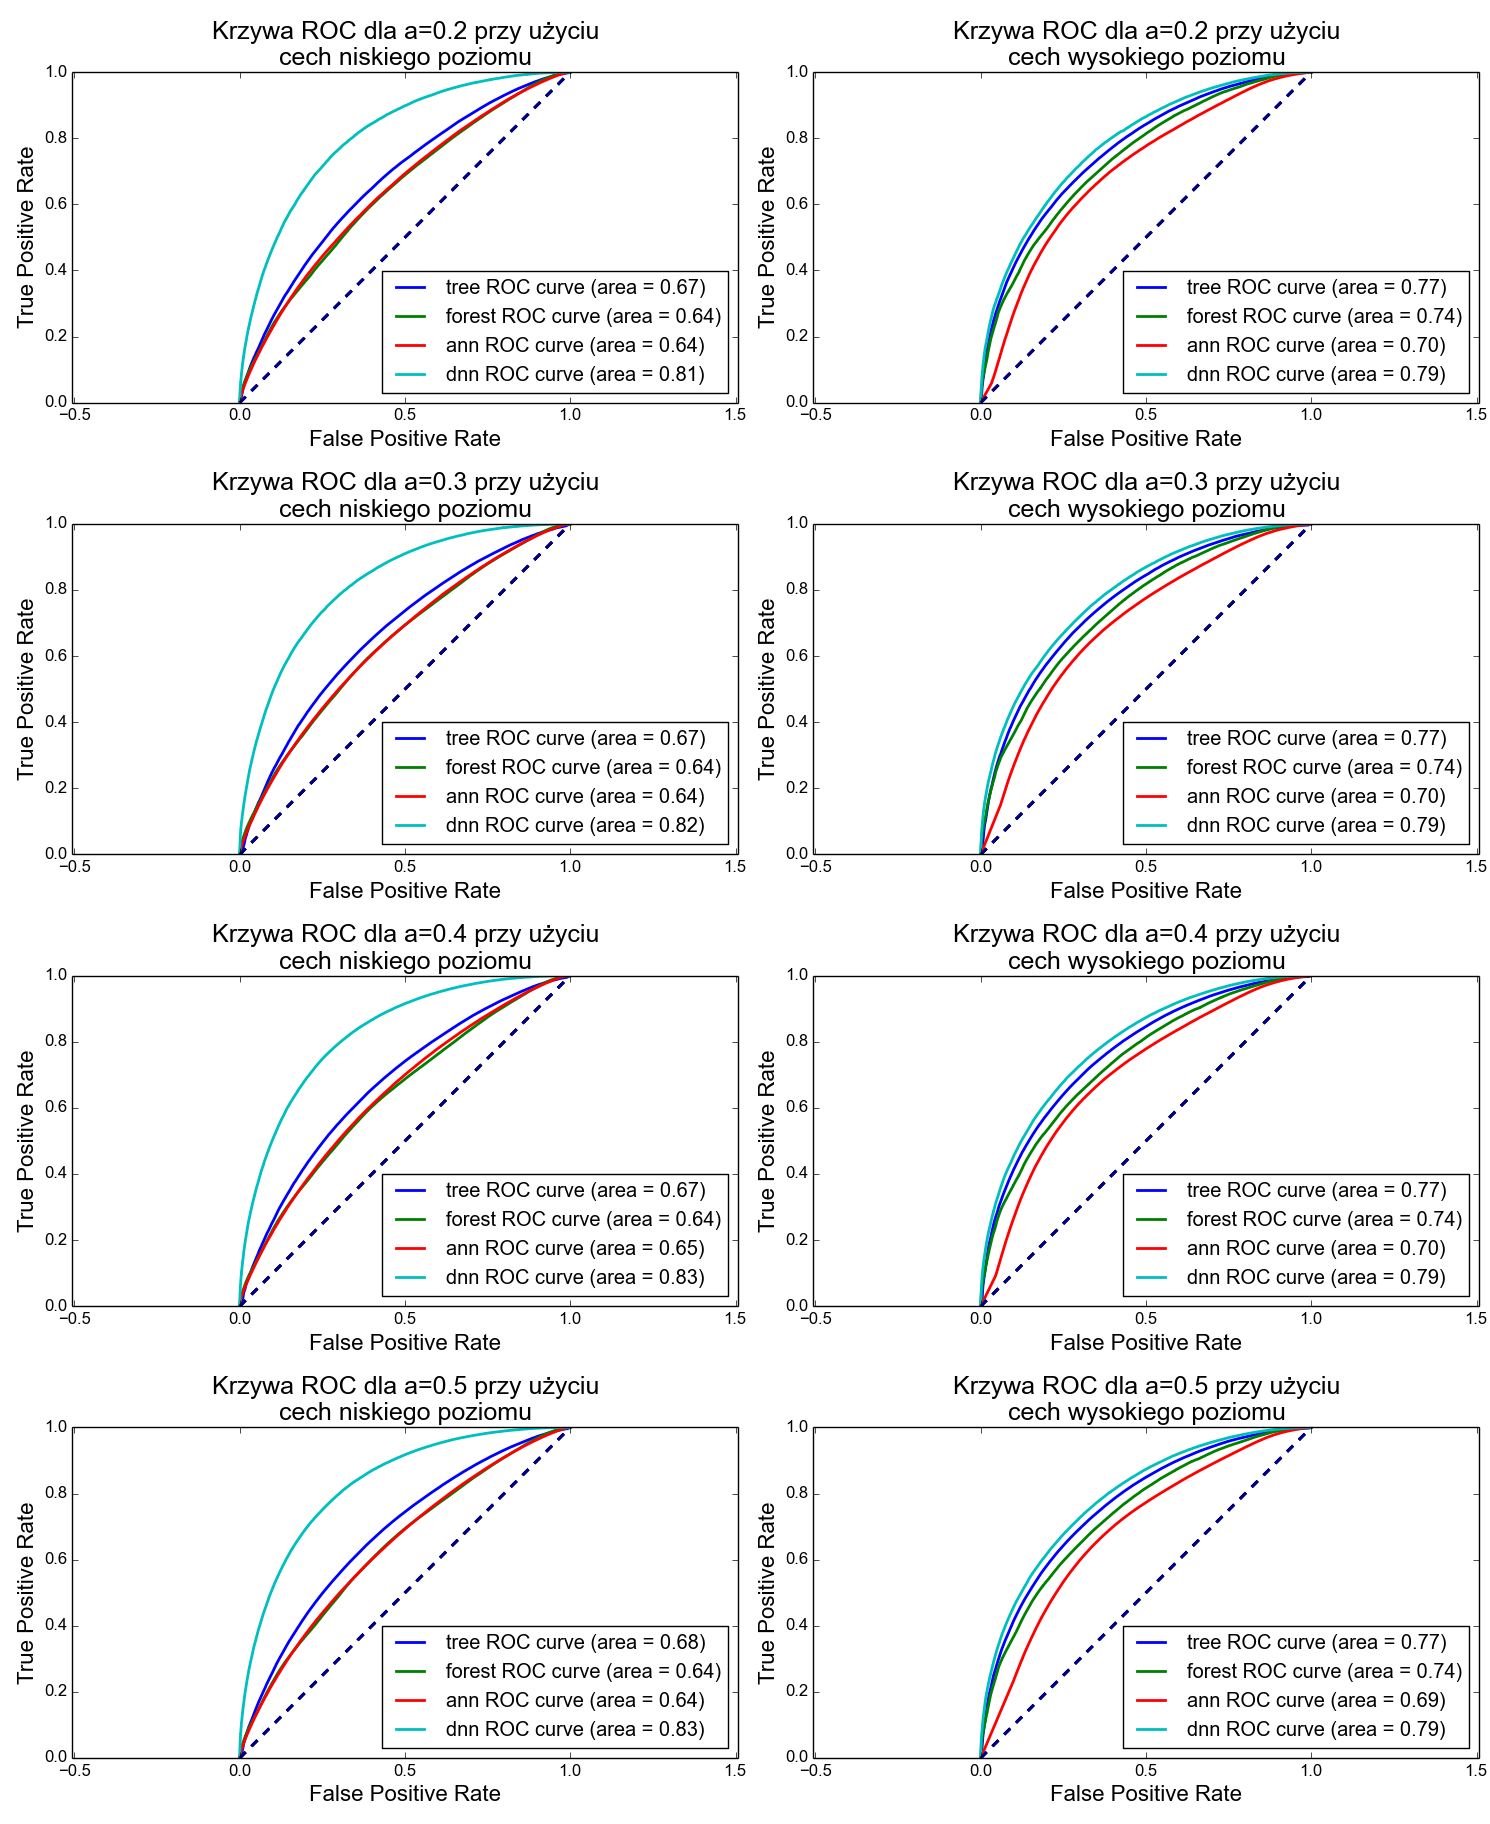
\includegraphics[scale=0.425]{res/allnew2.png}
\caption[Caption for LOF]{Krzywa ROC dla $a\in\{0.2, 0.3, 0.4, 0.5\}$\label{higgsall2}}
\end{figure} 

\begin{figure}[ht!]
\centering
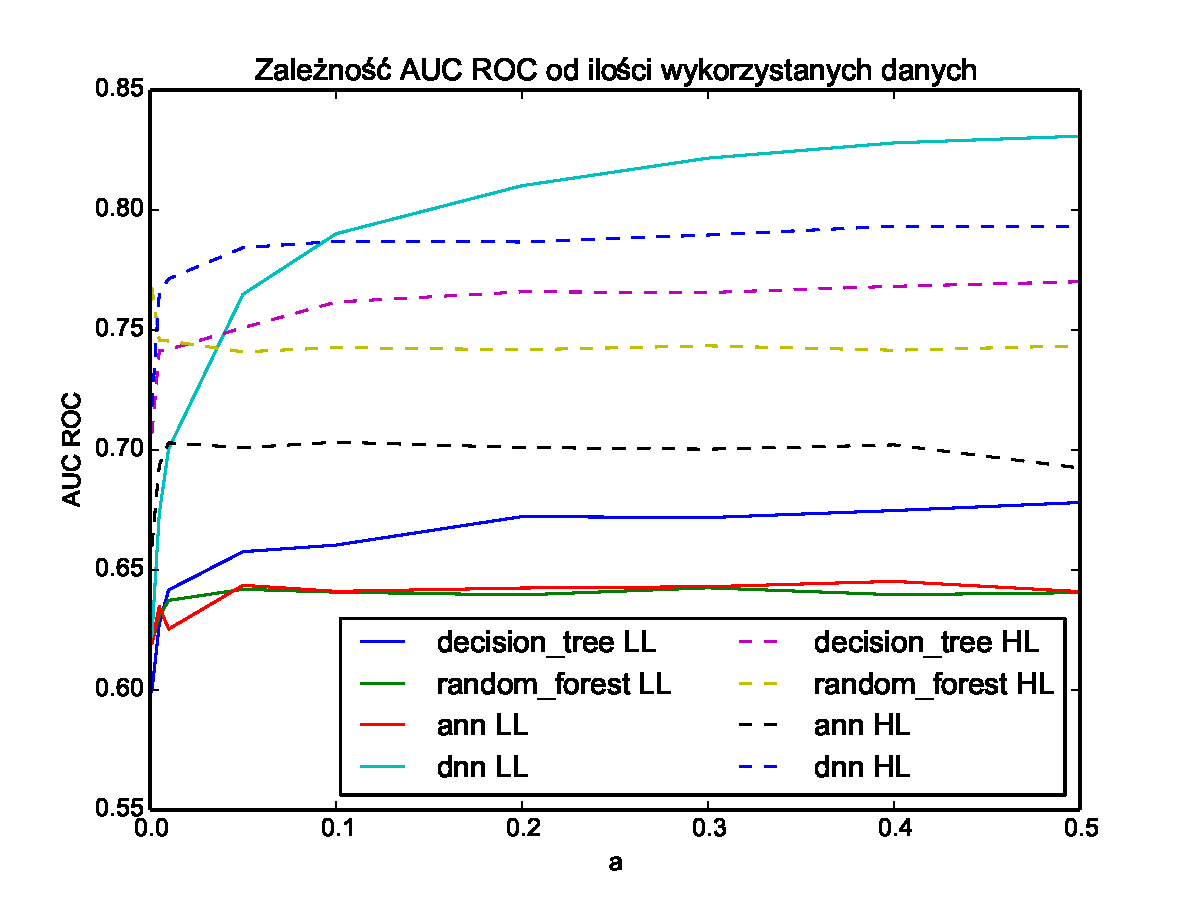
\includegraphics[scale=0.8]{res/higgssummary.pdf}
\caption[Caption for LOF]{Porównanie AUC ROC w zależności od rodzaju wykorzystanych cech dla wszystkich testowanych metod\label{higgssummary}}
\end{figure} 

\subsubsection{Wnioski}
Na~podstawie wykresu podsumowującego ten eksperyment, łatwo stwierdzić, że~w~przypadku wszystkich metod, przy użyciu mniejszej ilości danych uzyskane wyniki są znacznie lepsze w~przypadku wykorzystania cech wysokiego poziomu. Wraz ze~wzrostem liczby danych, skuteczność głębokich sieci neuronowych przy wykorzystaniu cech niskiego poziomu znacznie wzrasta i~szybko przewyższa wyniki innych metod niezależnie od~wykorzystanych atrybutów w~celu uczenia. W~przypadku, gdy $a=0.001$ najlepszy uzyskany wynik osiągnięty jest przy użyciu lasu drzew decyzyjnych (patrz tabela \ref{table:higgstable}). Stanowi to dowód na~to, że~w~przypadku niskiej liczby rekordów warto rozważyć ekstrakcje cech przy użyciu ,,wiedzy'' w~celu redukcji wymiarowości danych. Stwarza to możliwość użycia prostszych modeli uczenia maszynowego, które~są zdecydowanie łatwiejsze w~uczeniu w~przypadku, gdy dysponujemy niską ilością danych. Są one także bardziej odporne na~przeuczenie.

